%%%%%%%%%%%%%%%%%%%%%%%%%%%%%%%%%
% This is a slightly modified template of the one built by
% Steven V. Miller. Information can be found here:
%  http://svmiller.com/blog/2016/02/svm-r-markdown-manuscript/
%
% I added the use of raggedright to the anonymous option
% because journals,  the ability to put all the footnotes
% in endnotes, and the ability to manually adjust
% the starting page from the YAML header.
%
% Here are the options that you can define in the YAML
% header.
%
% fontfamily - self-explanatory
% fontsize - self-explanatory (e.g. 10pt, 11pt)
% anonymous - true/false. If true, names will be supressed and the
%                       text will be double-spaced and ragged
%                       right. For submission.
% endnotes - true/false. If true, the footnotes will be put in a
%                   section at the end just ahead of the references.
% keywords - self-explanatory
% thanks - shows up as a footnote to the title on page 1
% abstract - self explanatory
% appendix - if true, tables and figures will have  in
%                   front
% appendixletter - The letter to append to tables and figures in
%                             appendix
% pagenumber - Put in a number here to get a starting page number
%                         besides 1.
%%%%%%%%%%%%%%%%%%%%%%%%%%%%%%%%%%


\documentclass[11pt,]{article}
\usepackage[left=1in,top=1in,right=1in,bottom=1in]{geometry}
\usepackage{amsmath}
\usepackage{float}
\usepackage{dcolumn}

\newcommand*{\authorfont}{\fontfamily{phv}\selectfont}
\usepackage[]{mathpazo}


  \usepackage[T1]{fontenc}
  \usepackage[utf8]{inputenc}



\usepackage{abstract}
\renewcommand{\abstractname}{}    % clear the title
\renewcommand{\absnamepos}{empty} % originally center

\providecommand{\tightlist}{%
  \setlength{\itemsep}{0pt}\setlength{\parskip}{0pt}}

\renewenvironment{abstract}
 {{%
    \setlength{\leftmargin}{0mm}
    \setlength{\rightmargin}{\leftmargin}%
  }%
  \relax}
 {\endlist}

\makeatletter
\def\@maketitle{%
  \newpage
%  \null
%  \vskip 2em%
%  \begin{center}%
  \let \footnote \thanks
    {\fontsize{18}{20}\selectfont\raggedright  \setlength{\parindent}{0pt} \@title \par}%
}
%\fi
\makeatother




\setcounter{secnumdepth}{0}


\usepackage{graphicx}
% We will generate all images so they have a width \maxwidth. This means
% that they will get their normal width if they fit onto the page, but
% are scaled down if they would overflow the margins.
\makeatletter
\def\maxwidth{\ifdim\Gin@nat@width>\linewidth\linewidth
\else\Gin@nat@width\fi}
\makeatother
\let\Oldincludegraphics\includegraphics
\renewcommand{\includegraphics}[1]{\Oldincludegraphics[width=\maxwidth]{#1}}

\title{Disparities in Rural Indigenous Community Access to Healthcare in the
United States \thanks{Thanks to people and stuff}  }



\author{\Large Amanda Ricketts\vspace{0.05in} \newline\normalsize\emph{University of Oregon, Sociology}  }


\date{}

\usepackage{titlesec}

\titleformat*{\section}{\normalsize\bfseries}
\titleformat*{\subsection}{\normalsize\itshape}
\titleformat*{\subsubsection}{\normalsize\itshape}
\titleformat*{\paragraph}{\normalsize\itshape}
\titleformat*{\subparagraph}{\normalsize\itshape}


\usepackage{natbib}
\setcitestyle{aysep={}}
\bibliographystyle{./resources/ajs.bst}


%\renewcommand{\refname}{References}
%\makeatletter
%\renewcommand\bibsection{
%    \section*{{\normalsize{\refname}}}%
%}%
%\makeatother

\newtheorem{hypothesis}{Hypothesis}
\usepackage{setspace}

\makeatletter
\@ifpackageloaded{hyperref}{}{%
\ifxetex
  \usepackage[setpagesize=false, % page size defined by xetex
              unicode=false, % unicode breaks when used with xetex
              xetex]{hyperref}
\else
  \usepackage[unicode=true]{hyperref}
\fi
}
\@ifpackageloaded{color}{
    \PassOptionsToPackage{usenames,dvipsnames}{color}
}{%
    \usepackage[usenames,dvipsnames]{color}
}
\makeatother
\hypersetup{breaklinks=true,
            bookmarks=true,
            pdfauthor={Amanda Ricketts (University of Oregon, Sociology)},
             pdfkeywords = {keywords},
            pdftitle={Disparities in Rural Indigenous Community Access to Healthcare in the
United States},
            colorlinks=true,
            citecolor=blue,
            urlcolor=blue,
            linkcolor=magenta,
            pdfborder={0 0 0}}
\urlstyle{same}  % don't use monospace font for urls

\usepackage{endnotes}


\newlength{\normalparindent}
\setlength{\normalparindent}{\parindent}

%prettier captions for figures and tables
%I am making the text of figure captions smaller but not table captions
\usepackage[labelfont=bf,labelsep=period]{caption}
\captionsetup[figure]{font=footnotesize}

\begin{document}

% \pagenumbering{arabic}% resets `page` counter to 1
%


% \maketitle

{% \usefont{T1}{pnc}{m}{n}
\setlength{\parindent}{0pt}
\thispagestyle{plain}
{\fontsize{18}{20}\selectfont\raggedright
\maketitle  % title \par

}

{
   \vskip 13.5pt\relax \normalsize\fontsize{11}{12}
\textbf{\authorfont Amanda Ricketts} \hskip 15pt \emph{\small University of Oregon, Sociology}   

}

}







\begin{abstract}

    \hbox{\vrule height .2pt width 39.14pc}

    \vskip 8.5pt % \small

\noindent This is a test abstract


\vskip 8.5pt \noindent \emph{Keywords}: keywords \par

    \hbox{\vrule height .2pt width 39.14pc}



\end{abstract}


\vskip 6.5pt

\noindent  \hypertarget{introduction}{%
\section{Introduction}\label{introduction}}

Healthcare in the United States, while not restricted in variety, poses
several barriers for individual access to its services. Private
healthcare insurance provides the socially desired increase in choice of
options, but often results in higher out of pocket costs and deductibles
(Doonan et al.~2015). As a result, only the wealthy few with little to
no health issues benefit. Medicare additionally provides significant
choice, ``but also entails significant out-of-pocket costs for its
seniors and disabled beneficiaries'' (Doonan et al.~2015, 755). Medicaid
promises to give recipients open choice to providers, but the federal
government allows states to secure waivers to instead provide a limited
network (Doonan et al.~2015). Widespread use of Multiplan networks adds
another node of complication to understanding access and coverage. This
apparent limitless quantity of options has not, however, resulted in an
increase in the quality of care recipients receive. As of 2011, ``just
under one-quarter of the inhabitants of the more developed regions lived
in rural areas,'' and while urban centers are generally assumed to be
``less-healthy due to higher levels of overcrowding, air pollution, and
stress,'' they are in fact more healthy than their rural counterparts
(Hughes 2019). Rural communities, specifically rural Indigenous
communities in the United States, have unprecedented health disparities
and limited regularity of healthcare (Kruse et al.~2016).

In this study, I aim to measure the association between race and access
to healthcare, which will be quantified in health insurance coverage.
Specifically, I am asking to what extent do Indigenous populations in
the United States have access to healthcare, and how is this correlated
with urban versus rural status and employment? Recent studies have
criticized the overall biomedical approach of healthcare in the United
States that has ``developed over the last two centuries from
heteropatriarchal assumptions of women as reproducers,'' but few have
solely focused on Indigenous communities in the United States and
analyzed urban versus rural status as a higher level effect (Gurr 2014,
39). This interaction additionally has not taken into consideration the
Indian Health System, or IHS, which ``is a nationwide network of
hospitals and clinics that services 1.9 million American Indians and
Alaskan Natives who belong to some 564 tribes across 35 states with only
\$4.4 billion'' (Kruse et al.~2016, 1). The IHS operates independently
with limited resources, and the population served by this network have
exacerbated rates of type 2 diabetes, cardiovascular disease, and the
highest national rate of substance abuse (Kruse et al.~2016). Through
use of IPUMS census data, I will integrate these considerations into my
analysis of Indigenous access to healthcare.

\hypertarget{data-and-methods}{%
\section{Data and Methods}\label{data-and-methods}}

The data used in this study was sourced from IPUMS USA, an organization
that provides access to United States census data with enhanced
documentation. The data was accessed on May 5th via data extract
function on the organization's website. The sample includes 3,064
households and 6,405 individuals from 2017 to 2018, and it is
generalizable to the population of the United States. The data analysis
includes seven primary variables: age, narrowed from 18 to 65;
racecombo, which accounts for both race and ethnicity; marriage,
measured in either married or not married; employment, measured in
employed, non-employed, and not in labor force (NILF); anyhins, which
measures any health insurance coverage; metros, which addresses metro
status, measured as residence in a metro area, a non-metro area,
operationalized as rural, and mixed non-metro and metro status; and
finally, hins, which measures health insurance coverage through private,
IHS, public, and no coverage. Additional variables accounted for are
hhwt, cluster, strata, and perwt. These variables will be used to
account for clustering, stratification, and sampling weights. Future
analysis will include a consideration of design effects and models will
be weighted to account for proportions and cluster sampling. As such,
the following analysis is limited due to unequal proportions of race
representation in the studied data. Additionally, rurality cannot be
confirmed in the data, only non-Metro area residential status. Therefore
suburban and other non-rural areas have the propensity to be absorbed
into the non-Metro variable. The non-Hispanic American Indian Alaskan
Native variable is additionally unreliable due to non-representational
self-reporting; as a result, the results may be biased due to this.

\hypertarget{results}{%
\section{Results}\label{results}}

In the bar graph of metro area by race, I can see that a greater
proportion of NH AIAN reside in non-metro areas than both metro and
mixed areas. Whites are the majority in all residential areas, but
interestingly the greatest proportion of whites is found in non-metro
areas. In the Logit graph modeling the predicted probability of health
care coverage by race and age, I observe that an increase in the
predicted probability of health care coverage as age increases, but has
vastly different effects for race. In fact, a one year increase in age
beginning at age eighteen is associated with a 101.5\% increase in the
predicted probability health insurance coverage for whites, a 115.6\%
increase for Asian and Pacific Islanders, and only a 24\% increase for
American Indians and Alaskan Natives. AIAN have the lowest yearly
increase, 7.7\% below Hispanic individuals. In the predicted probability
of health care coverage by metro status and age graph, a one year
increase in age beginning at age eighteen is associated with a 102.0\%
increase in the predicted probability of health insurance coverage for
those in metro areas, a 71.2\% increase for mixed metro and non-metro
areas, and a 72.8\% increase in non-metro areas. Surprisingly, non-metro
areas have a slightly higher rate of predicted health insurance coverage
than mixed areas.

In the GLM Logit Model of Probability of Health Insurance Coverage by
Race and Metro Area, I can see that without holding any other
independent variables constant, non-Hispanic American Indians and
Alaskan Natives (NH AIAN) are predicted to be 4.2 times less likely to
have any health insurance coverage than whites. When holding constant
metro area, NH AIAN are 3.6 times less likely to have any health
insurance coverage than whites. When holding race constant, individuals
in non-metro, rural areas are 1.7 less likely to have any health
insurance coverage than their metro residing counterparts.
Interestingly, NH AIAN individuals in non-metro residential areas are
predicted to be 1.04 times more likely to have health insurance coverage
than non-metro whites. I hypothesize that this result is due to a higher
proportion of non-metro AIAN to metro residing AIAN than whites, and the
existence of the Indigenous-specific IHS health care system.

In the multinomial polytomous outcome model measuring the probability of
health insurance coverage by race, metro area, age, and employment,
holding all other variables constant, NH AIAN are predicted to have 3.2
times less health insurance coverage than whites. Hispanic individuals
are 3.5 times less likely, exceeding NH AIAN. Holding all other
variables constant, those who are not employed are predicted to be 1.9
times less likely to have health insurance coverage than employed
individuals. Additionally, holding all other variables constant, both
those in mixed metro areas and non-metro areas are predicted to be 1.6
times less likely to have health insurance coverage than metro area
residents. I therefore suggest than AIAN status is associated with a far
greater probability of having no health insurance than whites. Also,
non-metro and mixed metro status is associated with a far lower
probability of health insurance coverage than metro area residents.
Employment is additionally negatively correlated with health insurance
coverage.

\includegraphics{main_files/figure-latex/Boxplot Race and Metro Area-1.pdf}

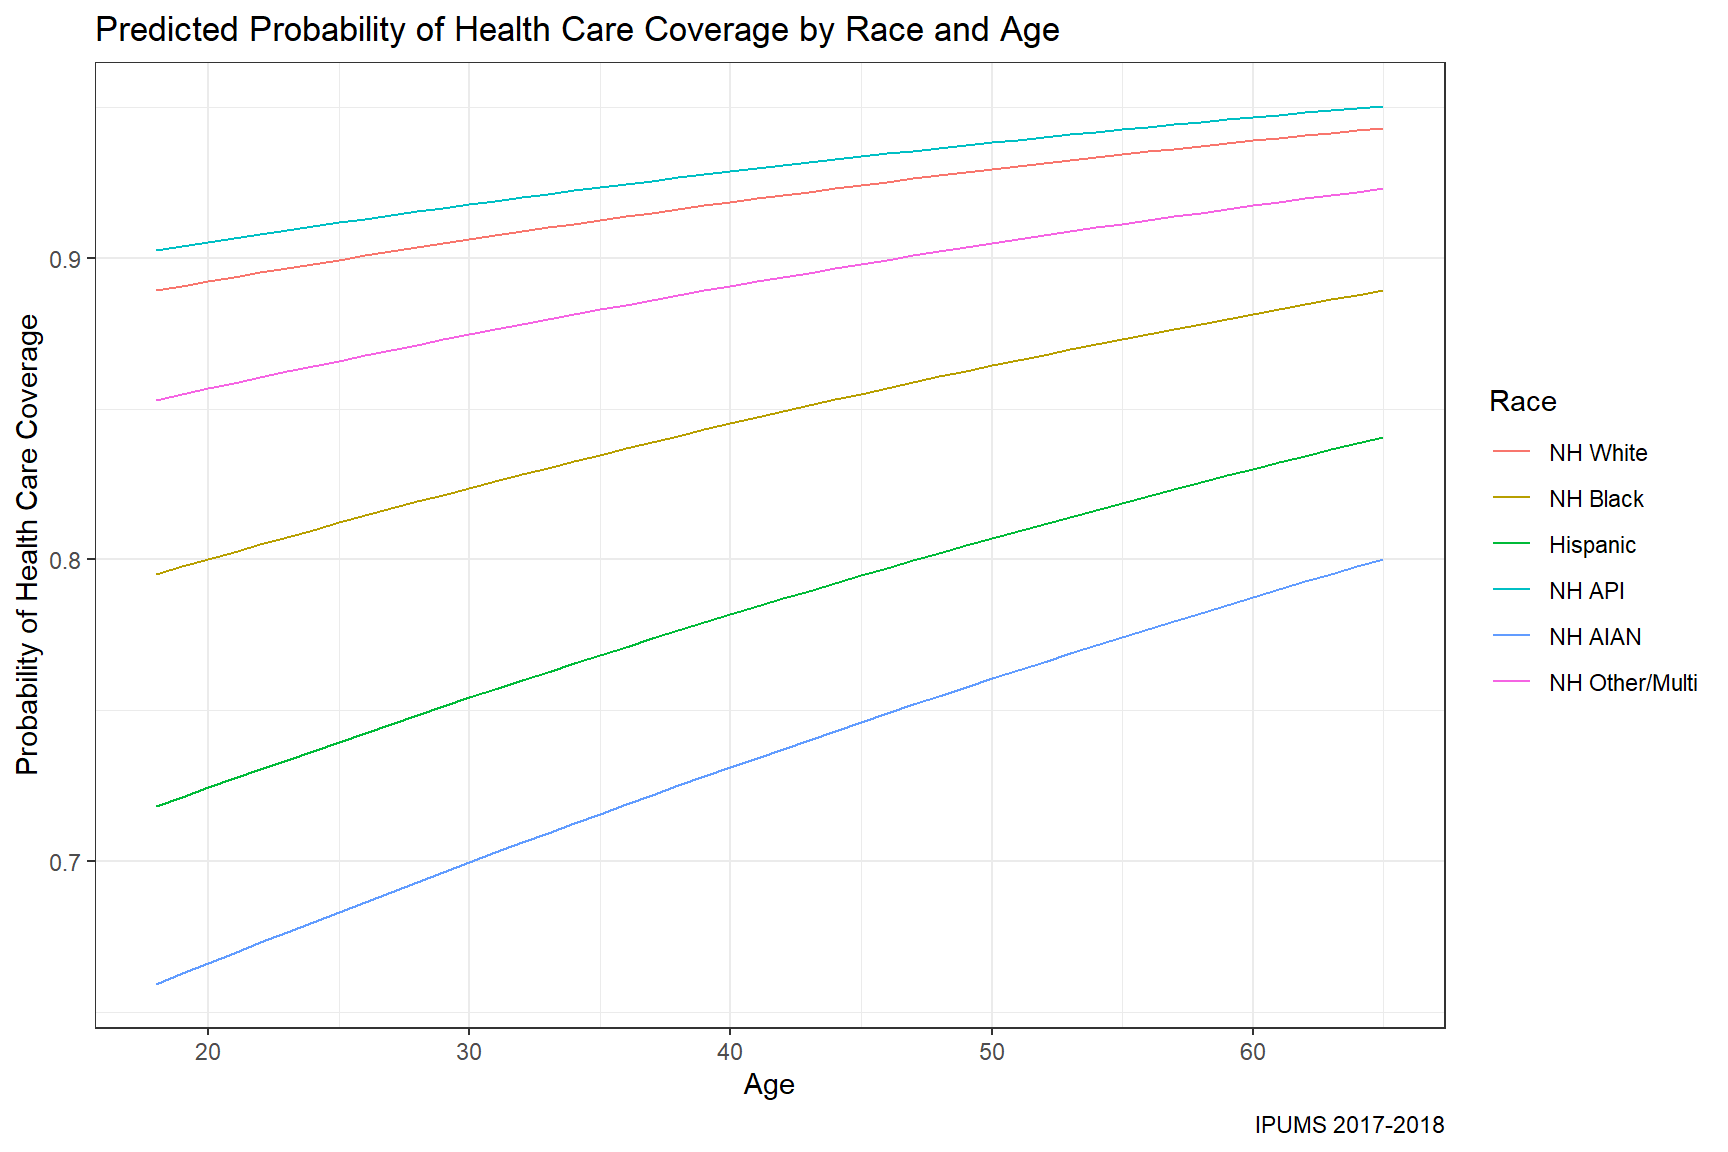
\includegraphics{main_files/figure-latex/Logit Race and Age Graph-1.pdf}

\begin{verbatim}
##             (Intercept)                     age       racecomboNH Black 
##               6.0747317               1.0156158               0.4835139 
##       racecomboHispanic         racecomboNH API        racecomboNH AIAN 
##               0.3173805               1.1558170               0.2409097 
## racecomboNH Other/Multi 
##               0.7221836
\end{verbatim}

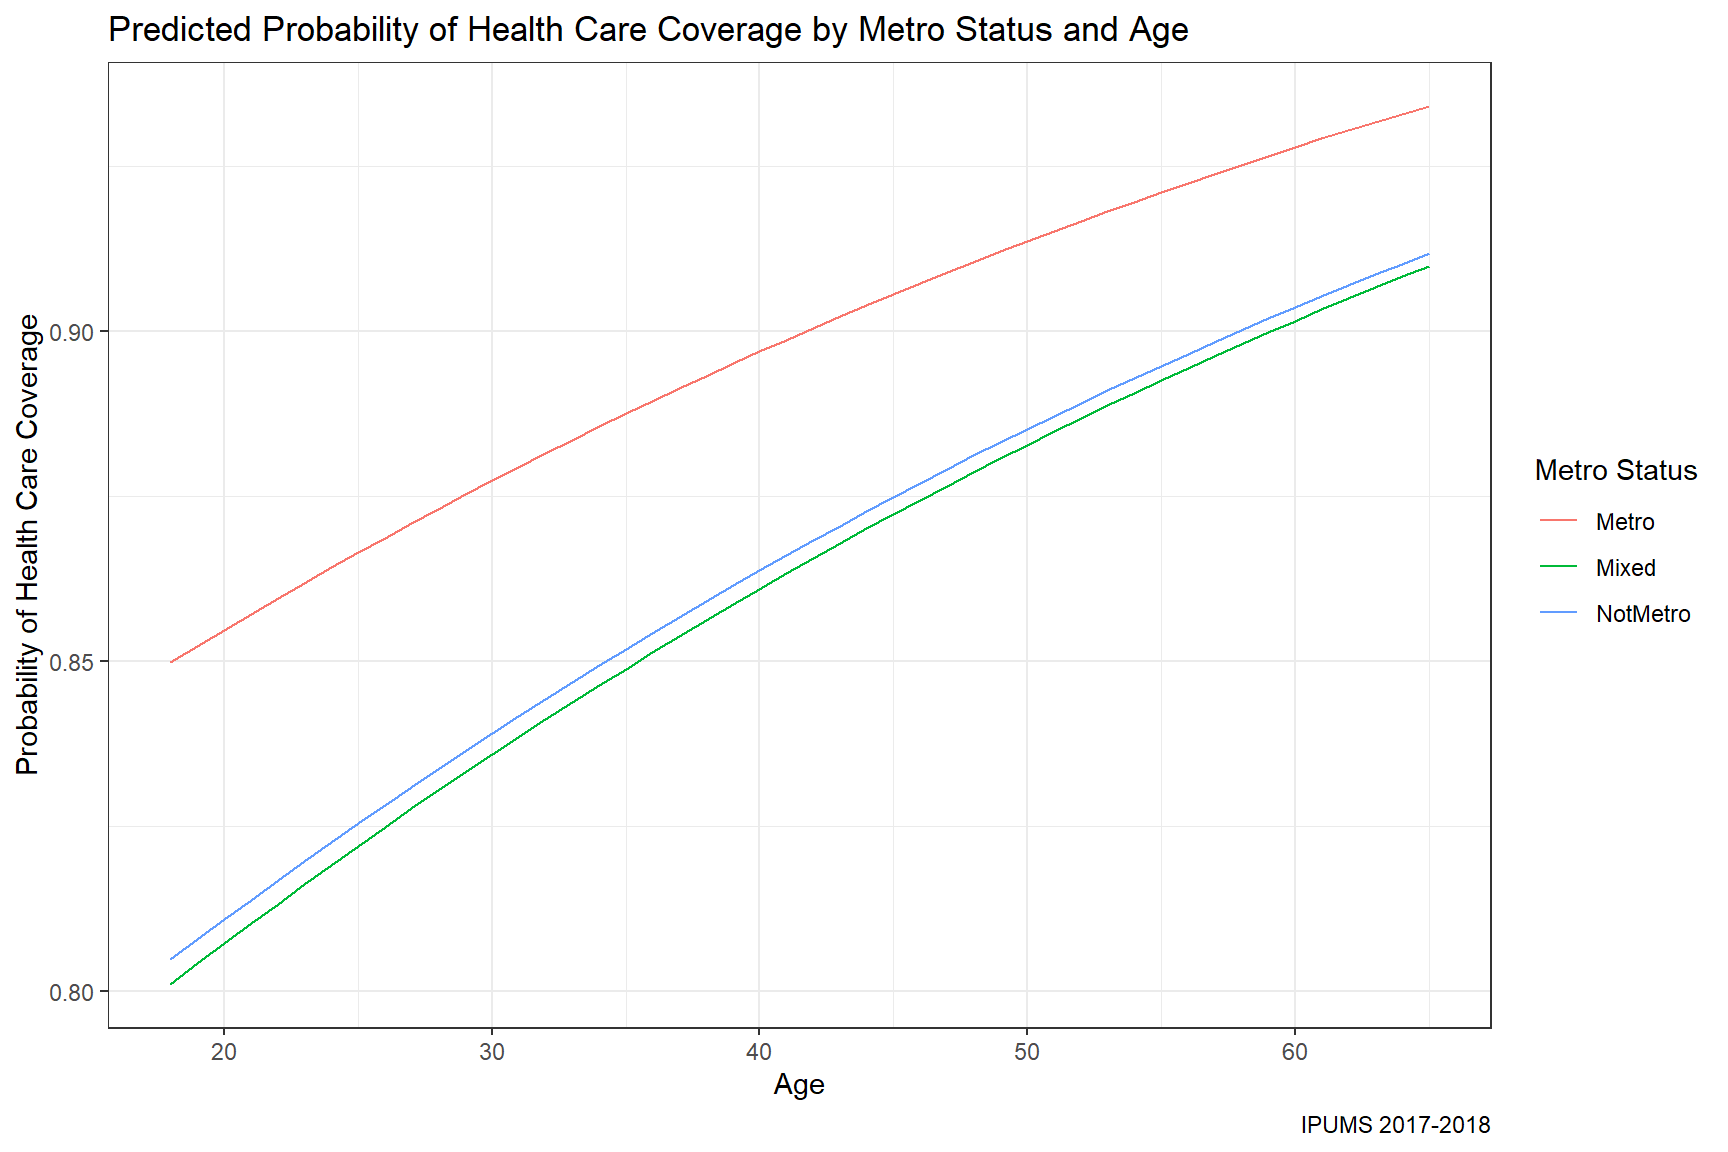
\includegraphics{main_files/figure-latex/Logit Metro Status and Age Graph-1.pdf}

\begin{verbatim}
##    (Intercept)            age    metrosMixed metrosNotMetro 
##      3.9783126      1.0197721      0.7115937      0.7284631
\end{verbatim}

\begin{table}
\caption{GLM Logit Model of Probability of Health Insurance Coverage by Race and Metro Area}
\begin{center}
\begin{tabular}{l c c c}
\hline
 & Model 1 & Model 2 & Model 3 \\
\hline
(Intercept)                            & $2.460^{***}$  & $2.636^{***}$  & $2.620^{***}$  \\
                                       & $(0.002)$      & $(0.003)$      & $(0.003)$      \\
racecomboNH Black                      & $-0.755^{***}$ & $-0.828^{***}$ & $-0.762^{***}$ \\
                                       & $(0.005)$      & $(0.005)$      & $(0.006)$      \\
racecomboHispanic                      & $-1.214^{***}$ & $-1.334^{***}$ & $-1.321^{***}$ \\
                                       & $(0.004)$      & $(0.004)$      & $(0.004)$      \\
racecomboNH API                        & $0.099^{***}$  & $-0.047^{***}$ & $-0.023^{**}$  \\
                                       & $(0.008)$      & $(0.008)$      & $(0.009)$      \\
racecomboNH AIAN                       & $-1.445^{***}$ & $-1.291^{***}$ & $-1.321^{***}$ \\
                                       & $(0.012)$      & $(0.012)$      & $(0.021)$      \\
racecomboNH Other/Multi                & $-0.423^{***}$ & $-0.483^{***}$ & $-0.427^{***}$ \\
                                       & $(0.011)$      & $(0.011)$      & $(0.013)$      \\
metrosMixed                            &                & $-0.526^{***}$ & $-0.484^{***}$ \\
                                       &                & $(0.005)$      & $(0.006)$      \\
metrosNotMetro                         &                & $-0.503^{***}$ & $-0.462^{***}$ \\
                                       &                & $(0.005)$      & $(0.006)$      \\
racecomboNH Black:metrosMixed          &                &                & $-0.201^{***}$ \\
                                       &                &                & $(0.014)$      \\
racecomboHispanic:metrosMixed          &                &                & $-0.042^{**}$  \\
                                       &                &                & $(0.013)$      \\
racecomboNH API:metrosMixed            &                &                & $-0.110^{**}$  \\
                                       &                &                & $(0.038)$      \\
racecomboNH AIAN:metrosMixed           &                &                & $0.017$        \\
                                       &                &                & $(0.030)$      \\
racecomboNH Other/Multi:metrosMixed    &                &                & $-0.220^{***}$ \\
                                       &                &                & $(0.030)$      \\
racecomboNH Black:metrosNotMetro       &                &                & $-0.332^{***}$ \\
                                       &                &                & $(0.017)$      \\
racecomboHispanic:metrosNotMetro       &                &                & $0.037^{*}$    \\
                                       &                &                & $(0.016)$      \\
racecomboNH API:metrosNotMetro         &                &                & $-0.229^{***}$ \\
                                       &                &                & $(0.048)$      \\
racecomboNH AIAN:metrosNotMetro        &                &                & $0.038$        \\
                                       &                &                & $(0.030)$      \\
racecomboNH Other/Multi:metrosNotMetro &                &                & $-0.143^{***}$ \\
                                       &                &                & $(0.036)$      \\
\hline
AIC                                    & $2610689.014$  & $2593168.818$  & $2592572.703$  \\
BIC                                    & $2610768.123$  & $2593274.296$  & $2592810.030$  \\
Log Likelihood                         & $-1305338.507$ & $-1296576.409$ & $-1296268.352$ \\
Deviance                               & $2610677.014$  & $2593152.818$  & $2592536.703$  \\
Num. obs.                              & $3932629$      & $3932629$      & $3932629$      \\
\hline
\multicolumn{4}{l}{\scriptsize{$^{***}p<0.001$; $^{**}p<0.01$; $^{*}p<0.05$}}
\end{tabular}
\label{table:coefficients}
\end{center}
\end{table}

\begin{verbatim}
## # weights:  11 (10 variable)
## initial  value 2725890.703668 
## iter  10 value 1300164.537846
## final  value 1271124.884424 
## converged
\end{verbatim}

\begin{verbatim}
##             (Intercept)       racecomboNH Black       racecomboHispanic 
##                 2.14580                -0.71512                -1.24697 
##         racecomboNH API        racecomboNH AIAN racecomboNH Other/Multi 
##                 0.02825                -1.16993                -0.34171 
##             metrosMixed          metrosNotMetro                     age 
##                -0.49817                -0.47141                 0.01614 
##   employmentNonemployed 
##                -0.62757
\end{verbatim}

\hypertarget{conclusions}{%
\section{Conclusions}\label{conclusions}}

In this study, I aimed to measure the association between race and
access to healthcare by asking the extent to which Indigenous
populations in the United States have access to healthcare, and how this
relationship is correlated with urban versus rural status and
employment. I hypothesized than non-metro areas would have less access
to healthcare than urban areas due to health disparities and lack of
access in the United States. I also applied this negative correlation of
access to NH AIAN communities, which are proportionately more rural than
whites. I preliminarily found that AIAN status is associated with a far
greater probability of having no health insurance than whites. Also,
non-metro and mixed metro status is associated with a far lower
probability of health insurance coverage than metro area residents.
Employment is additionally negatively correlated with health insurance
coverage, affirming my hypothesis. Further research needs to be done on
healthcare access across private, public, and IHS plans, specifically
how coverage from these different sources shifts between races and
across metro areas. Marriage status and employment additionally could be
more comprehensively addressed, and employment by urbanicity versus
rural status could present further findings. \# References

Dynamics under the Affordable Care Act.'' Current Sociology
63(5):746--62.

Gurr, Barbara. 2014. Reproductive Justice: The Politics of Health Care
for Native American Women. Rutgers University Press.

Hughes, Clarissa. 2019. ``Rural Health.'' Second Opinion: An
Introduction to Health Sociology 205--27.

Kruse, Clemens Scott, Shelby Bouffard, Michael Dougherty, and Jenna
Stewart Parro. 2016. ``Telemedicine Use in Rural Native American
Communities in the Era of the ACA: A Systematic Literature Review.''
Journal of Medical Systems 40(6):145.



\bibliography{../project.bib}
\end{document}
